\paragraph{}
After the geometry information is exported from the IGES file, it can be feed into the quad-tree algorithm to generate mesh of the problem domain.
As an algorithm based on computational geometry, it require great amount of numerical operation and hence the result may be sensitive to the tolerance.
An absolute tolerance may not be able to handle problem with very large or small geometric size.
As a consequence, the first step is to normalize the geometry into a uniform space ($10\times10$ is used in this chapter).

\subsection{Background mesh}
\paragraph{}
Background mesh, like its name, describe a mesh in the background. %fig
Its density is decided by the geometry.
This section will introduce the procedure to generate the background mesh.
\paragraph{}
First of all, we start with one square which is the root of the tree.
The size of it will be slightly larger than the normalized input geometry and it is selected as $16 \times 16$ in this chapter.
After that, the root square will be divided into millions (defined by resolution, defined as $2^{res} \times 2^{res}$) smaller ones like pixels in the image.
Then, $2^{s_{max}} \times 2^{s_{max}}$ ``pixels'' will be group into the first layer of the tree, or initial background mesh as shown in fig.~\ref{qdt_fig:qdt_initial_mesh}.
It is used to control the maximum allowable mesh size globally or separately for different material regions.

\begin{figure}[!ht]
    \centering
    \scalebox{0.8}{
        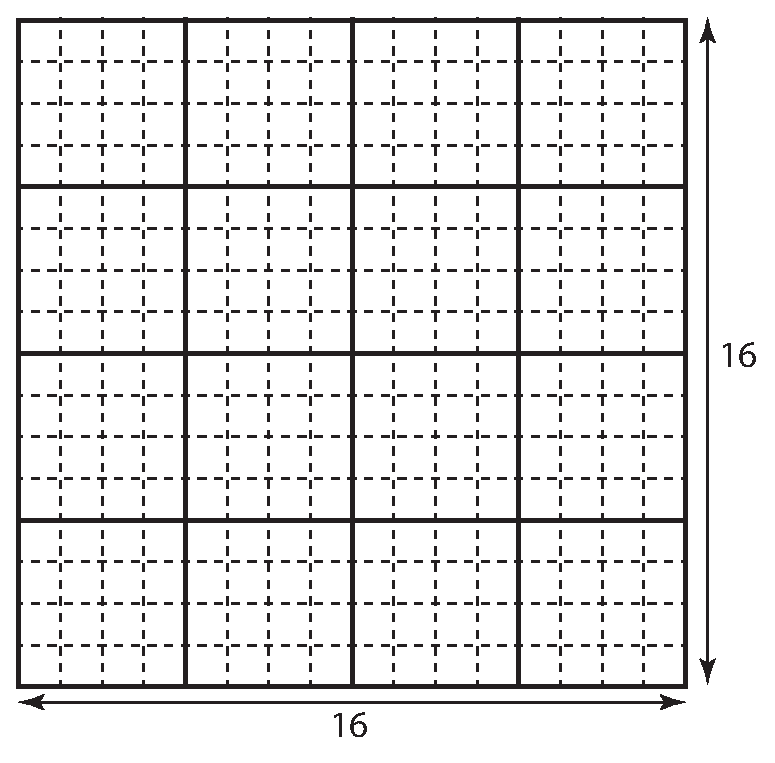
\includegraphics{quadtree/images/qdt_initial_mesh.eps}
    }
    \caption{An example of the background initial mesh: $16 \times 16$ square are divided into $2^4 \times 2^4$ pixels (dashed lines, $res=4$) and $2^2 \times 2^2$ pixels form the initial mesh (solid lines, $s_{max}=2$)}
    \label{qdt_fig:qdt_initial_mesh}
\end{figure}

\paragraph{}
% generating the initial mesh without balance
Criteria to decided whether each individual square in the initial mesh need to be refined or not is seed points.
The curve will be uniformly discretized into a given number of seed points uniformly and the mesh will be refined until the number of the seed points within the square is less than the threshold.
However, finer mesh is expected around the segment with high curvature in the curve and the uniform discretization does not emphasis on them.
It can be solved by treating each segment of the polylines as an individual curve when generating seed points.
Due to the fact that algorithm described in .~\ref{qdt_section:iges_output} guarantee the chord length to arc length ratio, polylines ought to have finer segments at the position where curvature is significant.

% balance the initial mesh
\paragraph{}
% balance in tree data structure
Self-balancing is adopted by most of the tree data structure such as AVL, B/B+, Red-black tree and so on.
Fig.~\ref{qdt_fig:tree_balance_avl} illustrates a self-balancing of an AVL tree.
Balancing by rotation is performed because difference in height of the leaf B and L is greater than the threshold.
    \begin{figure}
        \centering
        \scalebox{0.25}{
            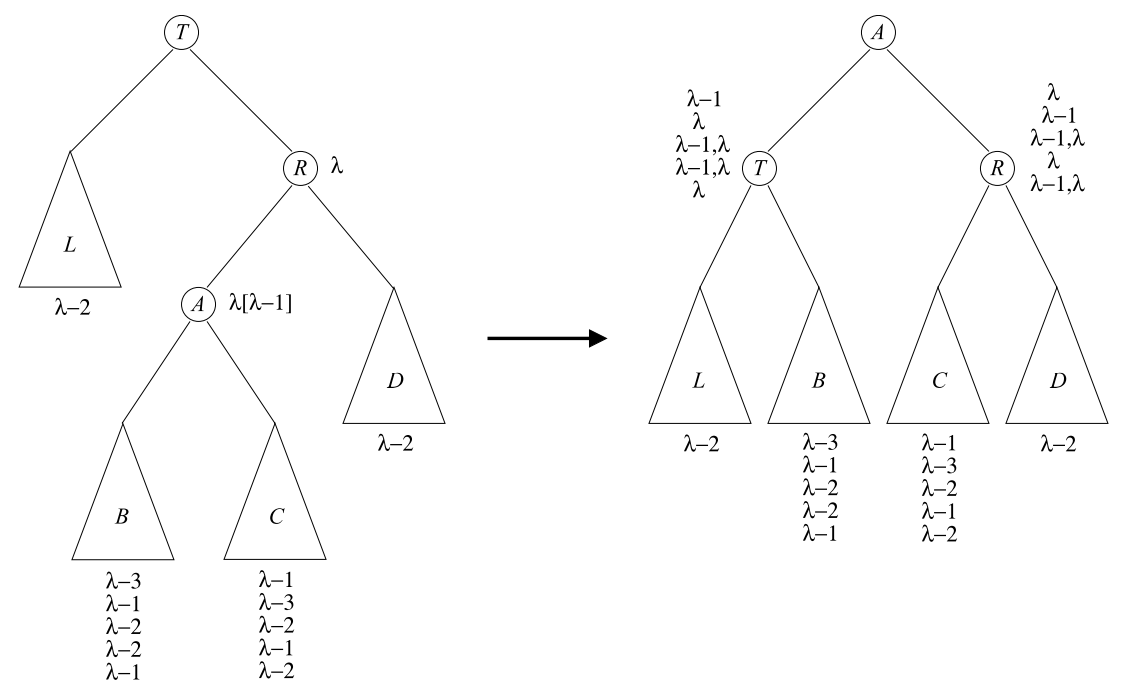
\includegraphics{quadtree/images/qdt_avl_balance.png}
        }
        \caption{Balance of the AVL tree \cite{Roura2013}}
        \label{qdt_fig:tree_balance_avl}
    \end{figure}

\paragraph{}
% balance in quadtree
Same idea is adopted in quadtree as well.
a refinement will be performed to achieve a balanced tree if the difference in the height of the leaf (Cell A and B in fig.~\ref{qdt_fig:tree_balance_quadtree} for example) is larger than one.
    \begin{figure}[!ht]
        \begin{subfigure}[b]{0.5\linewidth}
            \centering
            \scalebox{0.8}{
                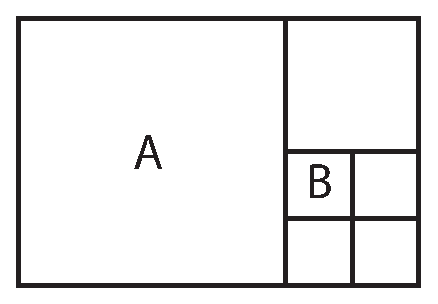
\includegraphics{quadtree/images/qdt_balance_before.eps}
            }
            \caption{Before balance operation}
        \end{subfigure}
        \begin{subfigure}[b]{0.5\linewidth}
            \centering
            \scalebox{0.8}{
                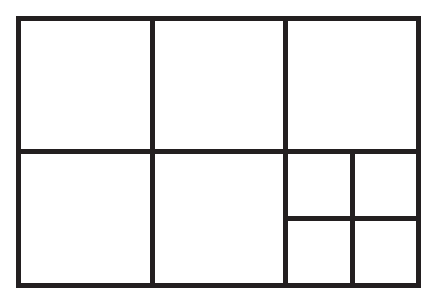
\includegraphics{quadtree/images/qdt_balance_after.eps}
            }
            \caption{After balance operation}
        \end{subfigure}
        \caption{Balance of quadtree: cell A is refined in order to balance the quadtree.}
        \label{qdt_fig:tree_balance_quadtree}
    \end{figure}

\paragraph{}
% reason behind balancing
The reason why balancing is predominately adopted in tree data structure lies in the guarantee of an $O\left(log(n)\right)$ time complexity for searching in any case.
Even thought computational cost on searching seems not to be significant during mesh generation using quadtree, a balanced tree provided some other attractive features that can be utilized in numerical analysis.
One of the advantages is to improve the mesh quality.
Any extremely small or large angle between the element and the scaling center may result in a bad quality mesh.
Chances are that these poor quality mesh may appear without self-balancing, fig.~\ref{qdt_fig:sbfem_adv_1} for an example.
    \begin{figure}[!ht]
        \centering
        \scalebox{1}{
            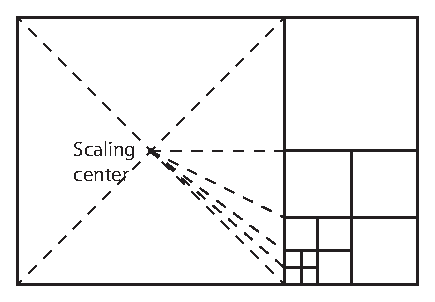
\includegraphics{quadtree/images/qdt_balance_sbfem_adv_1.eps}
        }
        \caption{Small angle between element and scaling center may reduce the mesh quality}
        \label{qdt_fig:sbfem_adv_1}
    \end{figure}

Another reason is to kept the pattern of the cells.
If the threshold of the self-balancing is set to one ($2:1$ ratio), only six kinds of cells will appear before the cutting as illustrated in fig.~\ref{qdt_fig:sbfem_adv_2}.
Thanks to the geometric similarity, local stiffness matrix can be calculated and scaled directly when same kind of the cell appears which significantly reduce the computational cost.
Hanging nodes in fig.~\ref{qdt_fig:sbfem_adv_2} can be a problem for traditional finite element to handle the displacement compatibility \cite{Tabarraei:2009:XFE} \cite{NME:NME3070} \cite{NME:NME2900} .
Solution including triangulation \cite{4037344} \cite{BERN1994384} \cite{ijeas251083} , using special shape function \cite{NME:NME1620120104} and other methods are available but special treatment is required.
As a comparison, SBFEM provides greater flexibility on the element, n-sides polygons with hanging nodes or curved edge can be treated natively.
    \begin{figure}[!ht]
        \centering
        \scalebox{1}{
            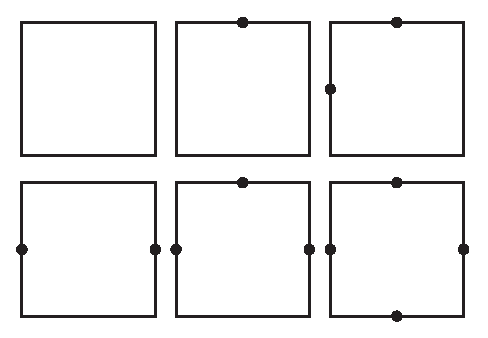
\includegraphics{quadtree/images/qdt_balance_sbfem_adv_2.eps}
        }
        \caption[Types of the cell in self-balancing quadtree]{
            Types of the cell when $2:1$ ratio is applied,
            \tikz\draw[black,fill=black] (0,0) circle (.7ex);
            stands for the hanging node
            }
        \label{qdt_fig:sbfem_adv_2}
    \end{figure}

%=====================================================================================================================%
\subsection{Hardpoint treatment}

%=====================================================================================================================%
\subsection{Bucket sort algorithm}

%=====================================================================================================================%
\subsection{Cutting with boundary}

%=====================================================================================================================%
\subsection{Color the region}
